Reading only 2 moves ahead on Arimaa requires at least \ensuremath{20 000^2 = 4 \times 10^8} positions to be explored. If the size of a node is 100 octets, in order to store such a tree, we would require \ensuremath{4\times10^{10} octets \approx 37,3 Gio}. Given the size of the data our software will be working on, it requires an efficient way of storing them. There are 2 kinds of data, on the one hand the ones the program works on, and on the other hand, the parameters and utilities.
\subsection{Representation of the playouts}
\subsubsection{Bitboards}
Boards are stored as bitboards. As the game is played on a \ensuremath{8\times8} board, it is convenient to use a 64 bit integer to store the position of the pieces. That way, each and every kind of piece is stored on the same x64 integer, saving space as opposed to a matrix \ensuremath{8\times8} retaining all the information. Players own rabbits, cats, dogs, horses, a camel and an elephant; thus using 6 integers for each player is the least . Adding a bitboard to store the position of every piece of each player helps to increase the speed of the algorithm by reducing the number of tests required, according to the playout phases. It also allows quick tests and modifications such as bit twiddling.% the nature of the data.

\subsubsection{Nodes}
\begin{figure}[H] 
\centerline{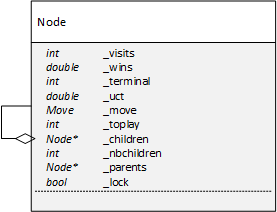
\includegraphics[scale=0.8]{Data_Structure/Img/Node.png}}
\caption{\label{fig:nodedetails}\textit{Details of the data cointained in a node}.}
\end{figure}
Nodes contains statistics on the previous results; a pointer to their parent; a pointer to the first of their children; and the number of children they own. They are stored in an array (\textit{\_tree}) set at the begining of the program, thus they are grouped on a countinuous memory segment. Therefore the time to gain access to them is decreased.

\subsubsection{Pruning}
Once a move has been played, only the sub-tree of its node is kept. The others have to be discarded in order to retrieve some memory. The process of removing these branches is called pruning.
\begin{figure}[H] 
\centerline{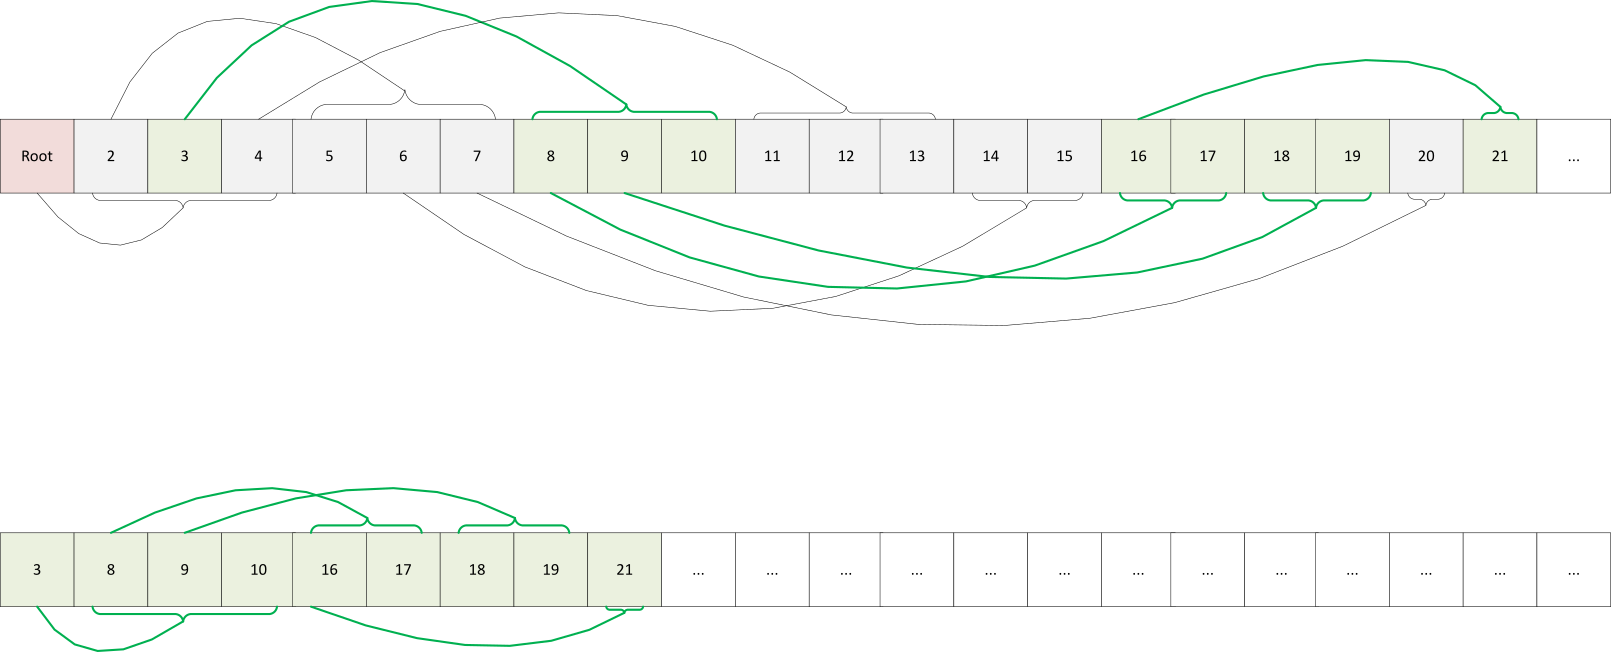
\includegraphics[width=\textwidth]{Data_Structure/Img/array.png}}
\caption{\label{fig:arrayprunning}\textit{Prunning of the tree (before and after)}.}
\end{figure}
In order to prune the tree, we use the following method : transform a copy of the current tree (\textit{\_tree}) into a buffer (\textit{\_buff}). The root of the buffer tree will be a copy of the node. Then the children are saved proceeding down through the branches. The advantage of this method is that you only copy the nodes you want to keep. However, the memory used by the buffer needs to be the same as that of the tree before the prunning. Thus, the maximum memory that can be used by the tree (\textit{\_tree}) is half the memory used by the program. In order to dermine the number of leaves to be created, the program checks how much memory there is left on the computer, and uses a fixed percentage of it.
\begin{equation}
N = \frac{R \times 90\%}{2}
\end{equation}
\ensuremath{N} = number of leaves.\\
\ensuremath{R} = RAM left to use.

We chose to limit the memory used by the tree to 90\% of the available memory in order not to overload the RAM and to leave some for other operations such as simulations. It also allows us to make sure that the swap will not be used to store the tree because it impacts heavily on the speed of its exploration capacities.

\subsubsection{Game abstraction}
\begin{figure}[H] 
\centerline{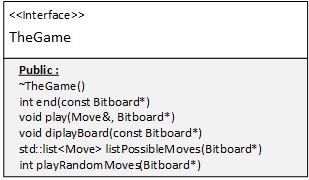
\includegraphics[scale=0.8]{Data_Structure/Img/TheGame.png}}
\caption{\label{fig:thegamedetails}\textit{Details of methods cointained in the interface TheGame}.}
\end{figure}
In order to know the moves that can be played and the winning conditions, the mcts algorithm has to have access to a class describing the game. This abstract class is implemented and passed as a parameter at the instantiation of the mcts object. It allows genericity in the algorithm and permits its use on any board games such as Connect4 or Arimaa. This interface has 4 main methods : 

\noindent
\textit{\textbf{end}} : check if the board provided is a final state.
\medskip\\
\textit{\textbf{play}} : play a given move on a given board.
\medskip\\
\textit{\textbf{listPossibleMoves}} : list all the possible moves on any given a board: this is used when a node is to be expanded.
\medskip\\
\textit{\textbf{playRandomMoves}} : play random moves until a final state is reached and a winner is returned. This is the random simulation part.

\newpage
\subsection{Parameters and utilities}
\subsubsection{Parameters}
Instead of directly passing all the parameters to the mcts object at its instantiation, we decided to create an object that would provide them using appropriate inline getters. The point of this is to allow quick modification on the parameters without having to rewrite some parts of the mcts to make sure that each file is updated. The main idea applied here is to separate the data from the algorithm using the same principle as the parameter object pattern.
\begin{figure}[H] 
\centerline{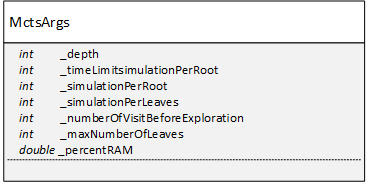
\includegraphics[scale=0.8]{Data_Structure/Img/MctsArgs.png}}
\caption{\label{fig:mctsargsuml}\textit{Details of the parameters of the algorithm}.}
\end{figure}

\subsubsection{Fast log}
The MCTS algorithm does not require an exact value of the \ensuremath{ln(x)} function in order to calculate the UCT value of a node. As binary numbers are stored on computers, it is more interesting to get their log in base 2 and to divide it by \ensuremath{ln(2)}. 
\begin{equation}
log2(x) = \frac{ln(x)}{ln(2)}
\end{equation}
\begin{equation}
ln(x) = log2(x) \times ln(2)
\end{equation}
\begin{equation}
ln(x) = log2(x) \times 0.69314718f
\end{equation}
Depending on the main operating system (Windows or Linux), the calculus of \ensuremath{log2(x)} will differ. On linux, a quadratic approximation is made. For further details, refer to annex \ref{subsec:fastLog}. On windows, \textit{\_BitScanReverse64(\&y, x)} is slightly faster. 

\subsubsection{Random numbers : Mersenne Twister}
Given the number of playouts to be simulated, the MCTS algorithm requires a fast random number generator. The Mersenne Twister which is implemented in the STL is faster than the basic rand() function. Therefore we decided to use it.


